\documentclass{article}
\usepackage[utf8]{inputenc}
\usepackage{graphicx}
\usepackage[margin=1in]{geometry}
\usepackage[dvipsnames]{xcolor}
\usepackage{amsmath} % needed for \text{...} in the equations
\usepackage{url}
\usepackage{hyperref}
\usepackage[numbers]{natbib} % for numeric references
\usepackage{titlesec}
% Tighter spacing so the report body fits in 2 pages
\titlespacing*{\section}{0pt}{1.4ex plus .5ex}{0.6ex}
\setlength{\textfloatsep}{8pt plus 2pt}
\setlength{\floatsep}{8pt plus 2pt}
\setlength{\intextsep}{8pt plus 2pt}
\setlength{\abovecaptionskip}{2pt}
\setlength{\bibsep}{0pt}

% The plots can sit next to this file (Overleaf) or one folder up (repository)
\graphicspath{{./}{../}}

\begin{document}

\begin{titlepage}
    \begin{center}
        % The logo comes with the Overleaf template; it is skipped if the
        % file is not there, so the report also compiles outside Overleaf
        \IfFileExists{figures/MSP-logo.jpg}{%
            \includegraphics[width=3cm]{figures/MSP-logo.jpg}}{}
        \vspace{1cm}

        {\LARGE\bfseries Where is the best instant ramen manufactured:\par}
        \vspace{0.3em}
        {\Large\bfseries A data driven comparison between countries and their product using public ramen reviews\par}

        \vspace{1.5cm}

        \textbf{\Large Frederique Mol (I6391802)}

        \vfill

        \large Date: \today

    \end{center}
\end{titlepage}

\newpage

\section*{Introduction}

Instant noodles are a staple household product that can be found in dozens
of countries, and the style, taste and quality can differ a lot between
producers.

Instant ramen was invented in Japan in 1958~\cite{cupnoodles}, and consumers and importers have often assumed that specific countries, such as Japan, produce the ``best'' instant ramen. A single average rating cannot settle this,
because an average based on few reviews is uncertain. In this report we test
the assumption with public review data and ask:
\textbf{Which country produces the best-rated instant ramen, and is the top
country's lead statistically meaningful?}

\section*{Data sample}
We use the \emph{Ramen Ratings} dataset published on
Kaggle~\cite{kaggle}, which is based on reviews by
\emph{The Ramen Rater}~\cite{ramenrater}. It contains 2{,}580 reviews, each of them reviewing a single instant-noodle product. The columns relevant to this analysis are:
\begin{itemize}
  \setlength\itemsep{0em}
  \item \texttt{Country}: country of manufacture (38 raw labels);
  \item \texttt{Stars}: rating from 0 to 5, mostly in steps of 0.25;
  \item \texttt{Brand}, \texttt{Variety}, \texttt{Style}: product
        information (355 brands; mostly packs, bowls and cups).
\end{itemize}
Three reviews marked \texttt{Unrated} were removed, which left us with
2{,}577 rated products. Country names were standardised: \emph{Holland}$\to$Netherlands,
\emph{Dubai}$\to$United Arab Emirates, \emph{United States}$\to$USA, and
\emph{Sarawak} (a Malaysian state)$\to$Malaysia. After this step we were left with 35 distinct countries.

\section*{Analysis method}
The analysis was written in base R and developed in VS Code. For each country
$c$ with $n_c$ reviews we computed the mean rating $\bar{x}_c$, the standard
deviation $s_c$ and the standard error of the mean
$\sigma_c = s_c/\sqrt{n_c}$. A mean based on only a few reviews is unreliable,
so only countries with $n_c \geq 10$ were kept (21 of 35 countries, which
covered a total of 2{,}514 reviews). These countries were then ranked by
$\bar{x}_c$. To decide whether two countries really differ, we treated their
means as independent and computed
\begin{equation}
  \Delta = \bar{x}_1 - \bar{x}_2, \qquad
  \sigma_\Delta = \sqrt{\sigma_1^2 + \sigma_2^2}.
\end{equation}
We call a difference significant if $\Delta > 2\sigma_\Delta$ (roughly a
95\% confidence level).

\section*{Results and discussion}
The average rating over all products is $3.65 \pm 0.02$ stars.
Figure~\ref{fig:top} shows the ten best-rated countries. Of the 21 countries
that pass the cutoff, the USA ranks 12th ($3.46\pm0.06$) and Canada is last
($2.24\pm0.20$).

\begin{figure}[!htb]
  \centering
  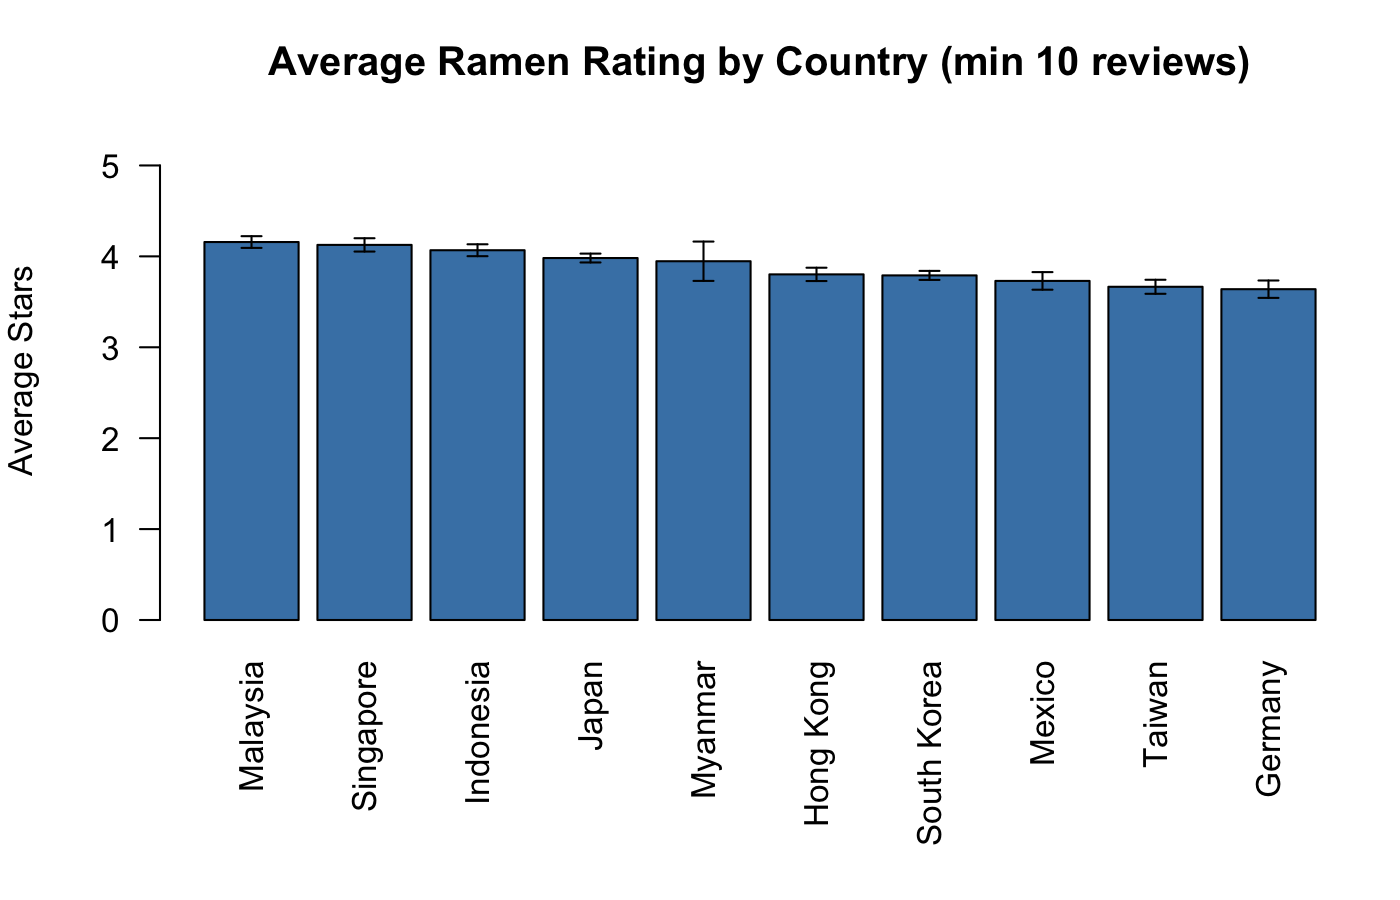
\includegraphics[width=0.5\textwidth]{ramen_top_countries.png}
  \caption{Mean star rating of the ten best-rated countries (at least 10
  reviews each). Error bars show $\pm1$ standard error of the mean.}
  \label{fig:top}
\end{figure}


Malaysia has the highest mean rating, followed closely by Singapore:
\[
  \bar{x}_{\text{Malaysia}} = 4.16 \pm 0.06, \qquad
  \bar{x}_{\text{Singapore}} = 4.13 \pm 0.07, \qquad
  \Delta = 0.03 \pm 0.10.
\]
The difference is only about $0.3\,\sigma_\Delta$, far below the
$2\sigma_\Delta$ threshold. \textbf{We therefore cannot say that Malaysian
ramen is better than Singaporean ramen: the two are statistically tied for
first place}, and Indonesia ($4.07\pm0.07$) is close behind. The top three
are all Southeast Asian countries. Japan, the country with the most reviews,
comes fourth ($3.98\pm0.05$). Its gap to Malaysia is
$\Delta = 0.18 \pm 0.08$, or $2.2\,\sigma_\Delta$, which is just above our
threshold. So the data do not support the assumption that Japan produces the
best-rated ramen. Myanmar, fifth ($3.95\pm0.22$), has the largest error bar
in Figure~\ref{fig:top}: its mean rests on only 14 reviews, all of products
from a single brand, with ratings spread from 2.75 to 5 stars. Its mean is
therefore poorly determined and consistent with Malaysia's
($\Delta = 0.21 \pm 0.23$, or $0.9\,\sigma_\Delta$).

In contrast, the spread across the whole ranking is large. With the same
method, the gap between Malaysia and the lowest-ranked country, Canada, is
$\Delta = 1.91 \pm 0.21$ stars, a difference of about $9\,\sigma_\Delta$. So the
country of origin clearly affects the rating, even though the best countries
cannot be separated from each other.

Figure~\ref{fig:scatter} shows the mean rating of every country against its
number of reviews, and it explains why the cutoff is needed. Without the cutoff,
Brazil ($4.35$ stars from only 5 reviews) would rank first and Nigeria
($1.5$ stars from a single review) last. Countries with many reviews lie closer to
the overall mean, yet Malaysia, Singapore and Indonesia remain about
$0.5$ stars above it with more than 100 reviews each. So their lead is not
a small-sample effect.

\begin{figure}[!htb]
  \centering
  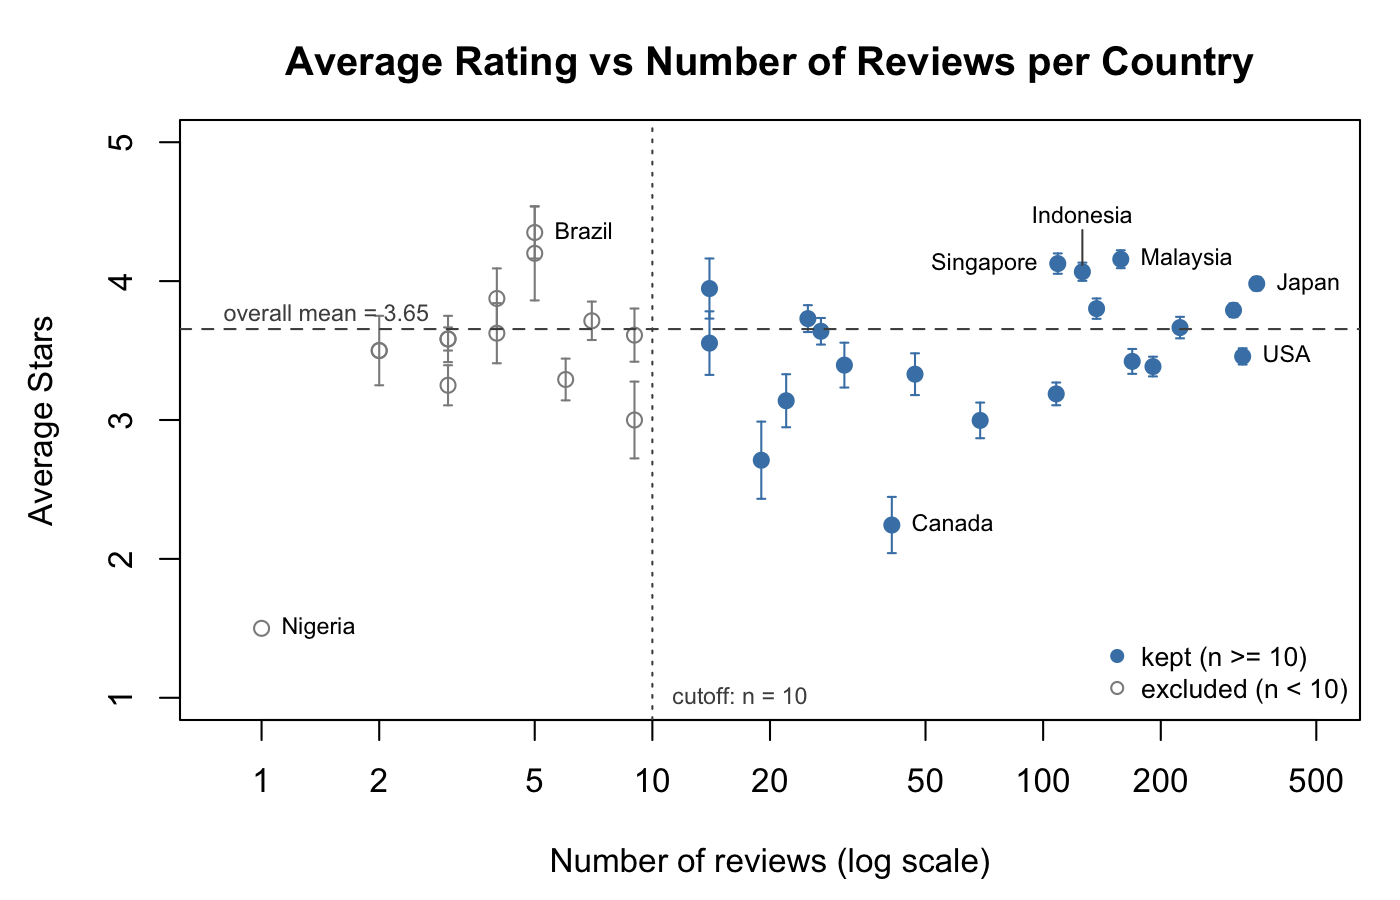
\includegraphics[width=0.52\textwidth]{ramen_rating_vs_reviews.png}
  \caption{Mean star rating against number of reviews for all 35 countries
  (log scale). Filled points pass the 10-review cutoff and open points are
  excluded. The dashed line is the overall mean. Error bars show $\pm1$
  standard error.}
  \label{fig:scatter}
\end{figure}

\section*{Conclusion}
The best-rated instant ramen comes from Malaysia ($4.16\pm0.06$ stars),
Singapore and Indonesia, about 0.5 stars above the overall average.
Malaysia's lead over Singapore ($0.03\pm0.10$ stars) is not statistically
meaningful, so there is no single best country. The country of origin does
matter, however: Malaysia is above Japan by $2.2\,\sigma_\Delta$ and above
Canada by $9\,\sigma_\Delta$. There are two limitations. All ratings come
from a single reviewer and the products were not sampled at random, which
the standard errors do not account for. And because we compare several pairs
of countries, a $2.2\,\sigma_\Delta$ result such as the Japan gap is only
weak evidence.

{\small
\begin{thebibliography}{9}
\bibitem{cupnoodles} CUPNOODLES MUSEUM OSAKA IKEDA, \emph{About}, n.d.
  \url{https://www.cupnoodles-museum.jp/en/osaka_ikeda/about/}
\bibitem{kaggle} A.~Bilogur, \emph{Ramen Ratings}, Kaggle. \url{https://www.kaggle.com/datasets/residentmario/ramen-ratings}
\bibitem{ramenrater} H.~Lienesch, \emph{The Ramen Rater: The Big List}.
  \url{https://www.theramenrater.com}
\end{thebibliography}}

\end{document}
